% ==== Types, layout, and lifetime ====
\section{Types, layout, and lifetime}

\begin{frame}{A quick reminder}
  \begin{itemize}
    \itemsep=1em
  \item C++ has fundamental + compound types (arrays, pointers, classes\ldots)
    \begin{itemize}
      \itemsep=1ex
    \item {\bfseries Class} types have {\bfseries base subobjects} and {\bfseries member subobjects}
      \begin{center}
        \tikz[byte/.style={draw,very thin,minimum width=14pt,minimum height=14pt,inner xsep=7pt},
                                start chain=c going right,node distance=0pt]{
\def\ptr#1#2{\draw[<-] (#1) -- ++(0pt,-10pt) node[at end,anchor=north] {#2};}

\node[on chain,font={\ttfamily\footnotesize}] {MostDerived};

\foreach \i in {0,...,3}
         \node[byte,fill=magenta!50!white!70,on chain=c] (i_\i) {};
\foreach \i in {0,...,3}
         \node[byte,fill=green!50!white!70,on chain=c] (f_\i) {};
\foreach \i in {0,...,7}
         \node[byte,fill=cyan!50!white!70,on chain=c] (d_\i) {};

\ptr{i_0.south west}{offset 0}
\ptr{f_0.south west}{offset 4}
\ptr{d_0.south west}{offset 8}

\node[below=25pt of d_0,font={\ttfamily},text width=4in]{
\begin{lstlisting}[style=c++,basicstyle={\ttfamily\footnotesize},backgroundcolor={}]
struct  Base { `\textcolor{magenta!50!white!70}{int i;}` }
struct  Derived : Base { `\textcolor{green!50!white!70}{float f;}` }
struct  MostDerived : Derived { `\textcolor{cyan!50!white!70}{double d;}` }
\end{lstlisting}
};
}

      \end{center}

    \item Types have size and {\bfseries alignment}!
    \end{itemize}
  \end{itemize}

  \begin{onlyenv}<2>
    \overlayLayer{
      \begin{itemize}
        \itemsep=1em
      \item Standard-layout \textit{[class.prop]}: TL;DR
        \begin{itemize}
          \itemsep=1ex
        \item All non-static members defined in same class
        \item All non-static members are also standard-layout
        \item No \inlineCode{virtual}
        \end{itemize}
        %
      \item POD: standard-layout + trivial
      \end{itemize}
    }
  \end{onlyenv}
\end{frame}

\begin{frame}{Storage Duration vs. Lifetime (1)}
  \begin{itemize}
    \itemsep=1em
  \item $Storage~Duration \neq Lifetime$!

  \item Storage Duration: \inlineCode{static}, \inlineCode{thread\_local}, automatic, dynamic
  \end{itemize}

  \vfill
  \begin{onlyenv}<1>
    \begin{block}{Lifetime starts\ldots%
        \hspace{24ex}\textit{[intro.object], par. 1}}
      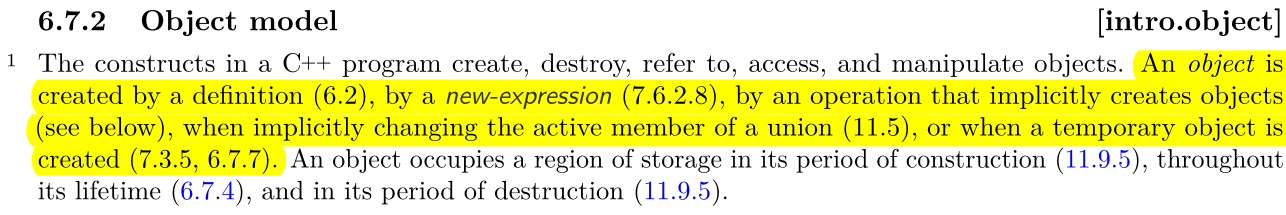
\includegraphics[width=\textwidth]{img/cplusplus_draft/intro.object.1.png}
    \end{block}
  \end{onlyenv}

  \begin{onlyenv}<2>
    \begin{block}{Lifetime ends\ldots%
        \hspace{24ex}\textit{[basic.life], par. 2.3--2.5}}
      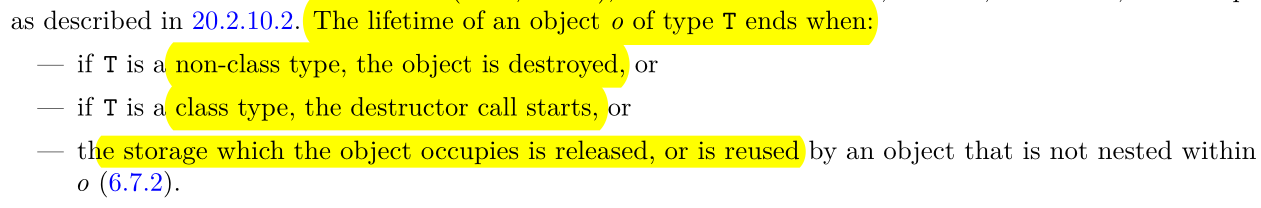
\includegraphics[width=\textwidth]{img/cplusplus_draft/basic.life.2.png}
    \end{block}
  \end{onlyenv}
\end{frame}

\begin{frame}[fragile]{Storage Duration vs. Lifetime (2)}
  \begin{lstlisting}[style=c++]
    using T = std::vector<int>;

    void *p = ::aligned_alloc(alignof(T), sizeof(T));
    static_cast<T*>(p)->push_back(101); // `\lsthl{UB!}`
``
  \end{lstlisting}  \vspace{-1em}%
  \pause%
  %
  \begin{lstlisting}[style=c++]
    auto v1 = new (p) T(); //    -\
    v1->push_back(42);     //     |- v1 vector lifetime
    v1->~T();              //    _/
    v1->push_back(102);    // `\lsthl{UB!}`
  \end{lstlisting}  \vspace{-1em}%
  \pause%
  \begin{lstlisting}[style=c++]
    auto v2 = new (p) T(); //    -\
    v2->push_back(123);    //     |- v2 vector lifetime
    v2->~T();              //    _/
    v2->push_back(103);    // `\lsthl{UB!}`
  \end{lstlisting}  \vspace{-1em}%
  \pause%
  %
  \begin{lstlisting}[style=c++]
    ::free(p);
  \end{lstlisting}

  \begin{onlyenv}<5>
    \overlayLayer{
      \bfseries Accessing an object out of its lifetime is UB\ldots\\[1em]
      \alert{\ldots even for trivial types!}
    }
  \end{onlyenv}
\end{frame}

\begin{frame}[fragile]{Implicit Lifetime (C++20)}
  Per C++20, objects may be created implicitly if it avoids UB\ldots\\[1em]

  \begin{lstlisting}[style=c++,caption=UB before C++20 (taken from P0593R6)]
    struct X { int a, b; };
    X *make_x() {
      X *p = (X*)malloc(sizeof(struct X)); // << C++20: implicitly create an X
      p->a = 1;
      p->b = 2;
      return p;
    }
  \end{lstlisting}

  \begin{onlyenv}<2>
    \tikz[remember picture,overlay]\node[at=(current page.center)]{\Huge\thinking\thinking\thinking};
  \end{onlyenv}

  \begin{onlyenv}<3>
    \overlayLayer{
      Happens in many places; remarkably:
      \begin{itemize}
      \item Memory allocation functions, incl. \texttt{malloc()}
        %
      \item \texttt{memcpy()} and \texttt{memmove()}
        %
      \item \texttt{std::bit\_cast()}
      \end{itemize}
    }
  \end{onlyenv}
\end{frame}

\begin{frame}{Alignment Requirements}
  Alignment determines which base addresses are legal for a data type.\\[1em]

  E.g. assuming \inlineCode{sizeof(int) == 4} and \inlineCode{alignof(int) == 4}
  \begin{itemize}
  \item An \inlineCode{int} may be at offset $0$, $4$, $8$, etc.

  \item But not at offset $3$
  \end{itemize}

  \begin{onlyenv}<2>
    \overlayLayer{
      \alert{\bfseries Important; underlying HW may be unable to do unaligned accesses.}
    }
  \end{onlyenv}
\end{frame}

\begin{frame}[fragile]{Padding / Packing}
  In order to ensure alignment, compiler may insert padding bytes
  \begin{lstlisting}[style=c++]
    struct X {
      unsigned char c;
      int i; /// <<<< Padding inserted before 'i'
    };
  \end{lstlisting}

  \vfill
  \begin{itemize}
    \itemsep=1ex
  \item Value of padding bytes is unspecified\ldots

  \item {\bfseries Packed structure:} do not include padding. \alert{Compiler-specific} ~~\NotOK
    %, e.g. \inlineCode{#pragma pack} or \inlineCode{\_\_attribute\_\_((\_\_packed\_\_))}
  \end{itemize}
\end{frame}
